\documentclass{standalone}
\usepackage{graphicx}	
\usepackage{amssymb, amsmath, amsthm}
\usepackage{color}

\usepackage{tikz}
\usetikzlibrary{intersections, backgrounds, math}

\definecolor{light}{RGB}{220, 188, 188}
\definecolor{mid}{RGB}{185, 124, 124}
\definecolor{dark}{RGB}{143, 39, 39}
\definecolor{highlight}{RGB}{180, 31, 180}
\definecolor{darkteal}{RGB}{29, 79, 79}
\definecolor{darkolive}{RGB}{97, 123, 45}
\definecolor{gray10}{gray}{0.1}
\definecolor{gray20}{gray}{0.2}
\definecolor{gray30}{gray}{0.3}
\definecolor{gray40}{gray}{0.4}
\definecolor{gray60}{gray}{0.6}
\definecolor{gray70}{gray}{0.7}
\definecolor{gray80}{gray}{0.8}
\definecolor{gray90}{gray}{0.9}
\definecolor{gray95}{gray}{0.95}

\tikzmath{
  function h(\x) {
    return 1.3 - 0.25 * \x - 0.5 * 9.806 * \x * \x;
  };
}

\begin{document}

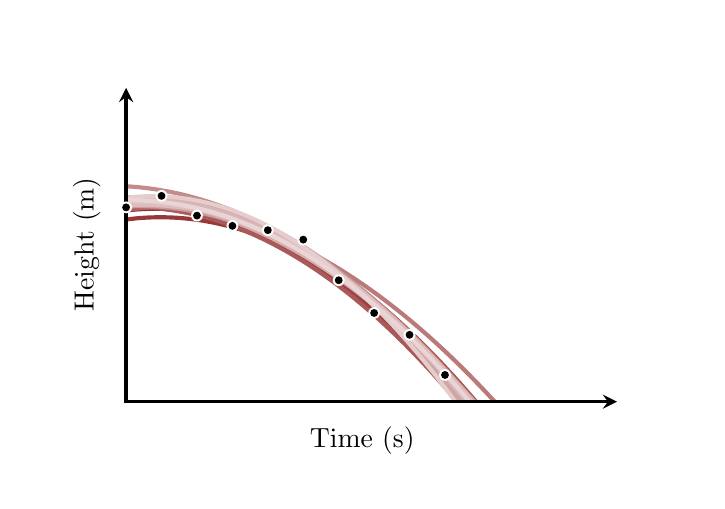
\begin{tikzpicture}[scale=1.0]
  
  \fill[white] (-4.25, -3) rectangle (4.25, 2.75);

  \begin{scope}
    \clip (-3, -2) rectangle (3, 2);
      
   \foreach \h/\v/\g [count=\n] in {1.227/0.283/11.489, 1.276/-0.131/10.229, 1.269/-0.128/10.405, 1.250/0.686/14.338, 1.214/0.535/12.827, 1.157/0.588/12.173, 1.298/-0.131/11.008, 1.232/0.402/11.945, 1.270/0.143/10.997, 1.235/0.080/11.648, 1.215/0.800/14.011, 1.237/0.358/12.308, 1.252/0.534/13.296, 1.239/0.143/9.708, 1.252/0.348/12.238, 1.368/-0.252/10.337, 1.265/0.299/12.399, 1.242/0.199/11.353, 1.262/0.660/14.095, 1.297/-0.274/9.617, 1.291/0.164/11.891, 1.245/0.318/11.746, 1.270/0.101/11.230, 1.295/0.535/14.280, 1.280/0.051/11.113} {
      \pgfmathsetmacro{\prop}{(100/ 26) * (30 - \n)};
      \colorlet{custom}{dark!\prop!white};
      \draw[domain={0:0.75}, smooth, samples=50, line width=1.5, variable=\t, color=custom] 
        plot ({9 * \t - 3}, { 2 * (\h + \v * \t - 0.5 * \g * \t * \t) - 2});
    }
  \end{scope}
  
  \draw [->, >=stealth, line width=1.25] (-3.00, -2.015) -- +(0, 4);
  \draw [->, >=stealth, line width=1.25] (-3.015, -2.00) -- +(6.25, 0);
  
  \foreach \t/\h in {0.0/1.23394124791483, 0.05/1.3070656869559456, 0.1/1.1816036167197874, 0.15/1.1164731174089624, 0.2/1.0891435492824528, 0.25/1.02924279648468, 0.3/0.7712501772229733, 0.35/0.5633948748371298, 0.4/0.4246340794176545, 0.45/0.16975557551895445} {
    \fill[white] ({9 * \t - 3}, { 2 * \h - 2}) circle (0.075);
    \fill[black] ({9 * \t - 3}, { 2 * \h - 2}) circle (0.050);
  }
  
  \node[rotate=90] at (-3.5, 0) { Height (m) };
  \node at (0, -2.5)  { Time (s) };
  
\end{tikzpicture}

\end{document}  
 